\documentclass[11pt,a4paper,twoside,asymmetric]{article}
\usepackage[english]{babel}
\usepackage{amsmath}
\usepackage{amsfonts}
\usepackage{amssymb}
\usepackage{graphicx}
\usepackage{float}
\usepackage{placeins}
\usepackage[left=3cm,right=2.5cm,top=3.5cm,bottom=2.5cm,%
headsep=0.75cm,headheight=2cm,footskip=1cm]{geometry}
\usepackage[dvipsnames]{xcolor}
\usepackage{fancyhdr}
\usepackage{tabularx}
\usepackage{booktabs}
\usepackage{titlesec}
\usepackage[labelsep=period]{caption}
\usepackage{multirow}
\usepackage{indentfirst}
\usepackage{xpatch}
\usepackage{setspace}
\usepackage{newtxtext}
\usepackage[labelfont=bf,font=small]{caption}
\captionsetup[table]{skip=6pt}

\usepackage{hyperref}
\hypersetup{
    colorlinks=true,
    linkcolor=RoyalBlue,
    urlcolor=RoyalBlue,
    citecolor=RoyalBlue,
    citebordercolor=0 0 1
    }
\urlstyle{same}

\addto\captionsenglish{\renewcommand{\figurename}{\textbf{\small{Fig.}}}}
\addto\captionsenglish{\renewcommand{\tablename}{\textbf{\small{Table}}}}

\titlespacing{\section}{0pt}{12pt}{4pt}
\titleformat{\section}[hang]{\large\bfseries}{\thesection. }{0.0em}{}

\titlespacing{\subsection}{0pt}{6pt}{3pt}
\titleformat{\subsection}[hang]{\bfseries}{\thesubsection. }{0.0em}{}

\renewcommand{\headrulewidth}{1.5pt}
\xpretocmd\headrule{\color{RoyalBlue}}{}{\PatchFailed}

\renewcommand{\footrulewidth}{1.5pt}
\renewcommand{\footrule}{\hbox to\headwidth{%
  \color{RoyalBlue}\leaders\hrule height \headrulewidth\hfill}}

\setlength{\parskip}{0.3em}
\raggedbottom
\widowpenalty=10000
\clubpenalty=10000
\renewcommand{\topfraction}{0.9}
\renewcommand{\textfraction}{0.07}
\renewcommand{\floatpagefraction}{0.7}
\setlength{\floatsep}{8pt plus 2pt minus 2pt}
\setlength{\textfloatsep}{10pt plus 2pt minus 2pt}

% Draft-only marker, same convention as paper/latex/main.tex: strip before submission.
\newcommand{\tbd}[1]{\textcolor{red}{[TBD: #1]}}
\newcommand{\needsapproval}[1]{\textcolor{OliveGreen}{[NEEDS AUTHOR APPROVAL: #1]}}

\fancypagestyle{firstpage}{
\fancyhf{}
\lhead{
\includegraphics[scale=0.15]{ijrcs}\\}
\rhead{
\includegraphics[scale=0.09]{ascee}\\}
\chead{International Journal of Robotics and Control Systems\\
\small{Vol. X, No. X, 2026, pp. X-X\\
ISSN 2775-2658\\
\url{http://pubs2.ascee.org/index.php/ijrcs}}}
\rfoot{
\includegraphics[scale=0.3]{email} \small{\href{mailto:ijrcs@ascee.org}{ijrcs@ascee.org}}}
\lfoot{
\includegraphics[scale=1]{doi} \small{\url{http://dx.doi.org/10.31763/ijrcs.v1i1.}}}
}

\fancypagestyle{followingpage}{
\fancyhf{}
\fancyhead[RE,LO]{\small{ISSN 2775-2658\\}}
\fancyhead[LE,RO]{\small{\textbf{\thepage}\\}}
\fancyhead[CE,CO]{International Journal of Robotics and Control Systems\\
\small{Vol. X, No. X, 2026, pp. X-X}}
\cfoot{\color{RoyalBlue}{\footnotesize{Duong, M. T. and Nguyen, P. H. (Multi-Backbone CCKD Reliability for Low-Electrode SSVEP BCI)}}}
}
\pagestyle{followingpage}
\AtBeginDocument{\thispagestyle{firstpage}}
\setcounter{page}{1}

\begin{document}
\begin{flushleft}
{\LARGE{
\begin{spacing}{1}
Cross-Channel Relational Knowledge Distillation for Low-Electrode SSVEP Brain--Computer Interfaces: A Multi-Backbone Reliability Study with Embedded Feasibility Assessment
\end{spacing}
}}
\vspace{1em}
Duong Mai Thuong $^{\text{a},1}$, Nguyen Phuong Huy $^{\text{b},2,\ast}$\\
\vspace{.5em}
\footnotesize{$^\text{a}$ Faculty of Information Technology, Thai Nguyen University of Information and Communication Technology, Thai Nguyen, Vietnam\\
$^\text{b}$ Faculty of Electronics Engineering, Thai Nguyen University of Technology, Thai Nguyen, Vietnam\\
$^1$ \textcolor{RoyalBlue}{duongmaithuong@tnu.edu.vn}; $^2$ \textcolor{RoyalBlue}{nguyenphuonghuy@tnut.edu.vn}\\
$^\ast$ Corresponding Author}
\end{flushleft}
{\color{RoyalBlue} \rule{\linewidth}{0.4mm}}
\vspace{.5em}
\noindent
\parbox[t][][s]{0.26\textwidth}{ARTICLE INFO
\vspace{.5em}

{\color{RoyalBlue}\rule{\linewidth}{0.4mm}}

\vspace{1em}
\footnotesize{\textbf{Article History}\\
\tbd{Received date}\\
\tbd{Revised date}\\
\tbd{Accepted date}\\
}

\vspace{1em}
\small{\footnotesize{\textbf{Keywords}\\
Steady-state visual evoked potential;\\
Knowledge distillation;\\
Brain--computer interface;\\
Centered kernel alignment;\\
Embedded deployment}
}
\vspace{.5em}
\vspace{\fill}
}
\parbox{0.025\textwidth}{\hspace{0.5em}}
\parbox[t][][s]{0.70\textwidth}{ABSTRACT
\vspace{.5em}

{\color{RoyalBlue} \rule{\linewidth}{0.4mm}}

\vspace{.5em}
\small{Reducing electrode count in a steady-state visual evoked potential (SSVEP) brain-computer interface improves wearability for wheelchair and speller applications but degrades decoding accuracy. Cross-channel relational knowledge distillation (CCKD) recovers part of this loss by transferring the relational structure of a multi-electrode teacher to a low-electrode student. This gain was reported previously for one backbone, FB-tCNN, on a single subject split. We extend that evaluation to five public backbones, two 40-target datasets (40 selectable stimulus frequencies each), and two student montages (electrode layouts). Each setting uses five independent subject splits and eight seeds per split. At a fixed distillation weight, only 2 of 20 backbone-dataset-montage settings remained significant after Holm-Bonferroni correction, both negative for EEGNet on BETA; neither survives at EEGNet's own validation-tuned weight, so no setting shows an effect robust to this routine hyperparameter choice. Single-split evaluation misjudged the sign or significance of the effect in 10 of 20 settings. Swapping the student montage flipped the sign in 12 of 40 cases. The accuracy gain correlated with the CCKD-induced increase in centered kernel alignment between teacher and student features (Pearson $r=0.55$, $p=0.012$). Distilling an intermediate layer together with the last layer matched or exceeded the better single-layer choice in 8 of 20 settings. Deploying the resulting students on a Raspberry Pi 4 and a Xilinx ZCU104 confirms post-quantization accuracy on both boards and inference latency well below an illustrative, unsourced control-loop budget. For the smallest backbone, synthesis onto the ZCU104's programmable logic (PL) succeeds within the board's resource budget, with on-board accuracy and latency matching expectations and board power that does not measurably exceed idle draw. These results show that cross-montage relational distillation is backbone- and montage-dependent, and that single-split evaluation is unreliable at the effect sizes typical of this literature.
}
\\
\\
\rightline{\footnotesize{\copyright~2026 The Authors.}}\\
\rightline{\footnotesize{Published by Association for Scientific Computing Electrical and Engineering.}}\\
\rightline{\footnotesize{This is an open access article under the \href{http://creativecommons.org/licenses/by-sa/4.0/}{CC-BY-SA} license.}}
\rightline{
\includegraphics[scale=1]{cc_by_sa}}}
{\color{RoyalBlue}\rule{\linewidth}{0.4mm}}

\section{Introduction}

A steady-state visual evoked potential (SSVEP) brain-computer interface (BCI) acts as the command-generation stage of a closed-loop control system: it senses the user's intent from EEG, maps the decoded target frequency to a discrete control command, and passes that command to a lower-level controller that actuates a wheelchair, a spelling interface, or a robotic arm \cite{R3,R6,R7,R8,R9}. As in any human-in-the-loop control architecture, the achievable command rate, measured in the BCI literature as the information transfer rate (ITR), sets the throughput of this channel. The decision latency of the classifier must also fit within the control loop's update period for the system to react safely to the operator's intent \cite{R4,R5}. A multi-electrode wet-gel cap improves decoding accuracy and therefore the reliability of each generated command. It also increases setup time and reduces wearability, which limits the use of such a controller outside the laboratory \cite{R39,R40,R41}. Reducing the electrode count to one or three channels improves wearability for a controller meant to be worn daily, but it degrades accuracy. The classifier loses the spatial information carried by the discarded channels, which in turn raises the rate of missed or incorrect commands sent to the actuator \cite{R36,R38}. This trade-off between the wearability of the sensing front end and the reliability of the control commands it produces is the central problem addressed in this paper.

Knowledge distillation (KD) offers one way to narrow this gap: a teacher network trained on the full montage transfers information to a student network restricted to the low-electrode layout \cite{R47}. Cross-channel relational knowledge distillation (CCKD) is one such method. It preserves the pairwise similarity structure of teacher features, encoded as a Gram matrix, instead of matching feature values directly \cite{R82}. In earlier work, we showed that CCKD recovers part of the accuracy lost to montage reduction for one convolutional backbone, FB-tCNN, on two public 40-target SSVEP datasets \cite{R82,R16}. That evaluation, like most EEG knowledge-distillation studies, used a single backbone, a single distillation layer, and a single subject split \cite{R48,R49,R50,R51,R52,R53}. This left open whether the benefit generalizes to other architectures, to other electrode subsets, or to a more rigorous multi-split evaluation.

SSVEP decoding has moved from spatial-filter methods such as canonical correlation analysis toward a wide range of deep architectures, including filter-bank convolutional networks \cite{R16}, transformer-based models \cite{R15,R23}, graph convolutional networks \cite{R18}, and attention-augmented compact networks \cite{R19,R20,R21,R26,R29}. These backbones differ in depth, receptive field, and the number of internal feature stages at which a teacher-student match can be imposed. A distillation strategy tuned for one architecture therefore need not transfer to another. A separate line of work shows that EEG machine-learning results are sensitive to how data are split and how significance is assessed: segment-level or single-split evaluation can invert the sign of an effect or inflate its apparent size \cite{R75,R76,R77,R78,R79,R80,R81}. Distillation gains reported in the sub-percentage-point range are exactly the regime in which this sensitivity matters most, yet our earlier CCKD evaluation relied on a single subject split \cite{R82}.

Centered kernel alignment (CKA) quantifies how similar two sets of neural-network representations are, independent of rotation and scale, and is a standard tool for comparing layers across trained networks \cite{R73,R74,R71,R72}. It matches the quantity that CCKD already optimizes, because the training objective matches the Gram matrix of pairwise sample similarities between teacher and student. CKA-based regularizers have been applied directly inside EEG backbones \cite{R70}. However, using the \emph{change} in CKA induced by distillation to predict how much accuracy the distillation step will recover remains untested in SSVEP decoding. Finally, deploying any of these backbones on the embedded hardware used in real wheelchair and speller prototypes, such as a Raspberry Pi 4 or a Xilinx FPGA, requires quantization and resource-aware implementation. This step can itself change classification accuracy \cite{R58,R60,R62,R63}. Whether a knowledge-distilled low-electrode model keeps its accuracy advantage after this step is a question the SSVEP-BCI literature has not addressed directly.

This paper extends our single-backbone conference evaluation \cite{R82} along four directions to close these gaps. The contributions of this research are as follows.
\begin{itemize}
\item[(i)] A controlled evaluation of CCKD across five public backbones (FB-tCNN, DeepConvNet, ShallowConvNet, EEGNet, and Compact-CNN), two 40-target datasets, and two low-electrode montages, each with five independent subject splits and eight seeds per split, with Holm-Bonferroni correction for multiple comparisons.
\item[(ii)] An analysis of centered kernel alignment between teacher and student features as a predictor of distillation benefit, including an intervention that distills an intermediate layer instead of the penultimate layer used in prior work.
\item[(iii)] A direct comparison of single-split and multi-split evaluation on the same data, quantifying how often single-split evaluation misjudges the sign or significance of the effect.
\item[(iv)] A deployment of the resulting student models on a Raspberry Pi 4 and a Xilinx ZCU104, the hardware classes used in wheelchair-control and SSVEP-speller prototypes, reporting decision latency against an illustrative control-loop update period (not sourced from a specific prototype), post-quantization accuracy, PL synthesis feasibility and on-board accuracy for the smallest backbone, and board-level power on the ZCU104 (the Raspberry Pi 4 has no on-board power sensor).
\end{itemize}

\section{Related Work}

\subsection{Deep Learning Backbones for SSVEP Decoding}
Classical SSVEP recognition relies on frequency-domain correlation methods, such as canonical correlation analysis and task-related component analysis, which compare the recorded signal against a reference template at each stimulation frequency. Convolutional and attention-based networks have since replaced or augmented these templates, achieving higher accuracy with less calibration data. FB-tCNN combines a filter bank with a time-domain convolutional network to handle short time windows \cite{R16} and is the backbone our 2026 conference paper distilled into a low-electrode student \cite{R82}. ConvCA replaces the fixed correlation template with a learned convolutional correlation layer \cite{R17}. SSVEPformer and related transformer architectures model long-range dependencies in the frequency-domain spectrum rather than the raw time series \cite{R15,R23}. Graph-convolutional variants such as DDGCNN exploit the spatial layout of electrodes directly \cite{R18}, and lightweight attention networks such as the task-attention model of Wang et al. and LGFCNN reduce the number of trainable parameters needed for individual calibration \cite{R20,R26}. Several studies address the few-channel regime directly, either through specialized architectures \cite{R22,R25,R38} or through analyses of how channel count and placement affect accuracy \cite{R36,R37}. Across this body of work, each architecture is typically evaluated and tuned on its own; comparative multi-backbone studies of any post-hoc transfer technique, including knowledge distillation, are rare.

\subsection{Knowledge Distillation for EEG and Brain-Computer Interfaces}
Knowledge distillation transfers information from a larger teacher network to a smaller or more constrained student network, usually by matching output logits, intermediate features, or pairwise feature relations. In EEG-based BCIs, similarity-keeping distillation reduces the channel count of a classifier while preserving most of its accuracy \cite{R47}. This is the closest precedent to the cross-channel relational objective evaluated in this paper. Other EEG and physiological-signal studies use distillation mainly across subjects or domains rather than across channel counts. Dual-teacher and multi-teacher frameworks combine several source models for motor-imagery decoding \cite{R49,R54}, teacher-assistant chains ease a large capacity gap between teacher and student \cite{R53}, and self-distillation or domain-generalization objectives target cross-subject and cross-dataset emotion recognition \cite{R50,R52,R55,R57}. A cross-modal variant distills knowledge from a visual encoder into an EEG encoder for continuous emotion recognition \cite{R51}. One study combines distillation with quantization-aware training in a single objective for EEG-based emotion recognition \cite{R56}, which anticipates the combined knowledge-distillation-and-embedded-deployment pipeline evaluated in this paper. None of these studies evaluate whether a channel-reduction distillation objective generalizes across backbone architecture, which is the first research question addressed here.

\subsection{SSVEP-Based Control Applications: Wheelchairs, Spellers, and Robotic Arms}
In an SSVEP-controlled assistive device, the decoder is one stage in a closed control loop. The stimulus interface presents a fixed set of flicker targets; the decoder maps the detected frequency to one discrete command out of that set; a low-level controller converts the command into a motion or selection primitive; and the device's motion, or the speller's screen feedback, closes the loop back to the operator. The number of commands available per unit time, and therefore the number of independent degrees of freedom the operator can control directly, is set jointly by the number of stimulus targets and the decoder's ITR \cite{R4,R5}. Wheelchair-control systems built on this loop use SSVEP alone for discrete heading commands \cite{R3,R6}, SSVEP combined with electrooculography \cite{R2} or P300 potentials \cite{R7} to add command channels, or SSVEP combined with computer vision and augmented reality \cite{R7,R8}. In the last design, the onboard perception system supplies continuous obstacle avoidance and the SSVEP channel supplies only the high-level heading command, which reduces the decoding accuracy and update rate the BCI stage must guarantee for safe operation. Systematic reviews of this application area report that most prototypes still use eight or more electrodes, in part because the stimulation and classification pipeline was developed for a research-grade cap rather than a long-wear consumer headset. The same reviews report that few prototypes state a closed-loop latency budget explicitly \cite{R10,R11}. Speller interfaces face the same loop with a much larger command set: encoding more target characters needs a larger stimulus set and a correspondingly higher perceptual workload per selection. This motivates paradigm designs that enhance the discriminability of each frequency and keep the per-character decision time bounded, such as frequency-enhanced row-column spellers \cite{R4} and adaptive spatial filtering \cite{R5}. Robotic-arm control shares the same channel-count trade-off at a finer grain. Reducing the montage improves comfort for extended operation, but it narrows the margin between target frequencies that the decoder can resolve reliably. This directly limits how many independent joint or end-effector commands the control loop can safely accept \cite{R9}. These applications motivate the two deployment scenarios evaluated later in this paper: a three-electrode montage intended for a wheelchair headset, and a comparison across electrode subsets relevant to speller and robotic-arm command sets.

\subsection{Representation Similarity and Centered Kernel Alignment}
Centered kernel alignment (CKA) measures how similar two sets of representations are, without requiring the same number of units or a fixed correspondence between them. The Gaussian and linear variants of this measure have become standard tools for comparing layers across trained networks \cite{R73,R74,R71}. Kriegeskorte and Wei situate CKA within the broader framework of representational geometry, which compares the relative distances or similarities among stimuli rather than their absolute feature values \cite{R72}. This framework matches the quantity CCKD already optimizes. The training objective matches the Gram matrix of pairwise sample similarities between teacher and student, which is the same object CKA uses to quantify representational similarity. Tobon-Henao et al. apply a centered-alignment regularizer directly inside an EEGNet classifier for motor-imagery discrimination \cite{R70}, confirming that CKA-based objectives are compatible with EEG backbones. To our knowledge, no prior SSVEP study has used the change in CKA induced by distillation as a predictor of how much accuracy the distillation step recovers. This is the second research question addressed here.

\subsection{Statistical Reliability in Cross-Subject EEG Evaluation}
EEG classification accuracy is sensitive to how training, validation, and test data are partitioned across subjects and sessions. White and Power show that k-fold cross-validation without subject-level separation substantially overestimates accuracy in passive BCI designs \cite{R75}. Del Pup et al. and Kamrud et al. report that subject-wise partitioning choices alone change measured performance by several percentage points in cross-subject deep-learning models \cite{R76,R79}. Brookshire et al., Lee et al., and Geethapriya and Pattabiraman document the same leakage pattern in translational and clinical EEG classifiers. There, segment-level splitting lets a classifier exploit subject identity instead of the intended signal \cite{R77,R78,R81}. Xu et al. show that accuracy estimates also vary across different EEG datasets collected under nominally the same paradigm, independent of any single-subject leakage \cite{R80}. These findings motivate evaluating CCKD on five independent subject splits with Holm-Bonferroni correction, rather than on the single split used in the original conference evaluation. They also motivate the direct single-split-versus-multi-split comparison reported as the third research question of this paper.

\subsection{Quantization and Embedded Deployment for Real-Time BCIs}
In a control loop, the decoder's execution time is part of the loop's dead time: it adds directly to the delay between the operator's intent and the actuator's response. An embedded implementation must therefore keep that delay within the margin the mechanical system can tolerate without instability or a perceptibly sluggish response. Deploying a trained SSVEP classifier on embedded hardware for this kind of real-time, untethered operation typically requires quantization, pruning, or a dedicated hardware accelerator. A floating-point convolutional network otherwise exceeds the memory and power budget of a wearable or battery-powered controller. Pacini et al. compare CPU, GPU, and FPGA deployments of a motor-imagery CNN and report large differences in latency and power across platforms for the same trained model. This shows that the choice of compute platform, not only the model, sets the achievable control-loop rate \cite{R60}. Novac et al. provide a general methodology for quantizing and deploying deep networks on microcontrollers \cite{R63}. Palumbo et al. demonstrate a full FPGA-embedded BCI pipeline for locked-in patients, with the decoder running on the same board that generates the output command \cite{R62}. Spiking and event-driven architectures offer an alternative low-power path for wearable physiological-signal classification, demonstrated for ECG and seizure detection on FPGA \cite{R64,R65,R66,R67,R68,R69}. A recent survey catalogs edge-AI accelerator designs for brain-computer interfaces specifically \cite{R58,R61}. None of this work evaluates whether a knowledge-distilled student model, already trained to approximate a larger teacher, retains its accuracy advantage after the additional accuracy loss introduced by embedded quantization. Nor does it establish whether the student's latency on this class of hardware fits the control-loop budget required by a wheelchair or speller controller. This motivates the fourth research question addressed in this paper.

\subsection{Summary and Research Gap}
Across these five areas, three gaps motivate the present study, all bearing on the same practical question: can a low-electrode, knowledge-distilled SSVEP decoder serve as the command-generation stage of a real wheelchair, speller, or robotic-arm control loop without an unacceptable loss of command reliability or an unacceptable increase in decision latency? First, cross-channel knowledge distillation for SSVEP decoding has been evaluated on a single backbone. Its generalization across architecture, and therefore across the different embedded platforms that implement each architecture, is unknown. Second, no predictor of distillation benefit has been tested for this setting. Yet centered kernel alignment is readily available for this purpose and could guide which backbone-montage pair to deploy in a given control application. Third, the methodological risks documented for EEG cross-subject evaluation, including single-split overestimation, have not been applied to knowledge-distillation studies specifically. The embedded feasibility of the resulting student models, including whether their decision latency fits a realistic control-loop budget, has not been measured directly. The remaining sections of this paper address each gap in turn. Section 3 describes the backbones, datasets, and distillation protocol. Section 4 reports, in sequence, the multi-backbone and montage results, the CKA analysis and the layer-intervention experiment, the single-split-versus-multi-split comparison, and the embedded deployment results, relating decoder latency and accuracy to the control-loop requirements of the wheelchair and speller use cases introduced above. Section 5 concludes.

\section{Method}

\subsection{CCKD}
\label{sec:cckd}

\begin{figure}[htbp]
\centering
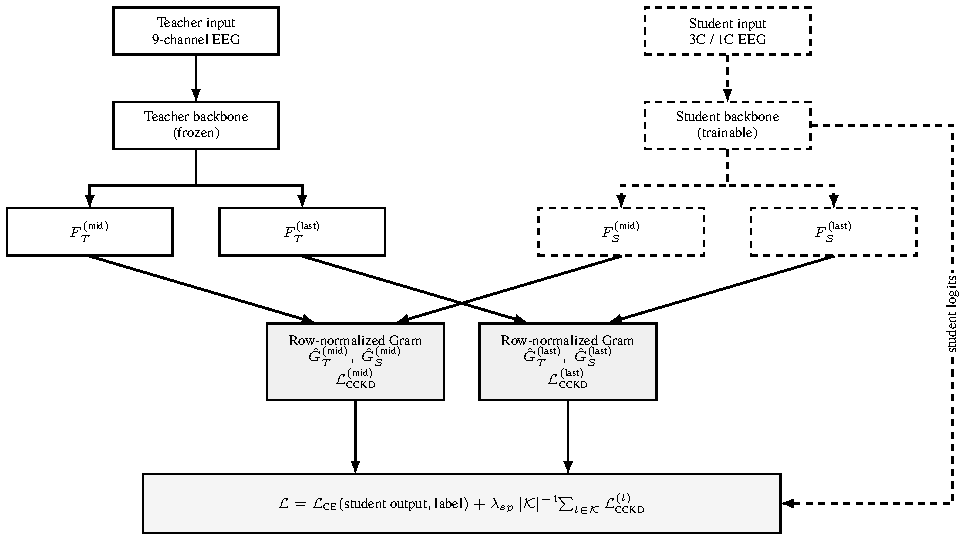
\includegraphics[width=\linewidth]{figures/method_overview.pdf}
\caption{Block diagram of CCKD. The fixed teacher (blue, solid) and the trainable student (green, dashed) both output features at the \texttt{mid} and \texttt{last} layers; each layer computes a row-normalized Gram matrix, which is then matched by $\mathcal{L}_{\text{CCKD}}$ (red). The total loss $\mathcal{L}$ adds the student's cross-entropy loss.}
\label{fig:method}
\end{figure}
\FloatBarrier

Figure~\ref{fig:method} summarizes the CCKD architecture described below. The teacher receives input from nine parieto-occipital electrodes, is pretrained with cross-entropy, and is then kept fixed. The student shares the teacher's architecture but receives only three or one electrode. For a mini-batch of $N$ samples, let $F_T^{(l)} \in \mathbb{R}^{N \times d_T}$ and $F_S^{(l)} \in \mathbb{R}^{N \times d_S}$ denote the teacher and student features at layer $l$. The Gram matrix of each model is $G^{(l)} = F^{(l)} (F^{(l)})^{\top} \in \mathbb{R}^{N \times N}$; because the Gram matrix always has size $N \times N$, CCKD does not require $d_T = d_S$. Each row is normalized by its $\ell_2$ norm, $\hat{G}^{(l)}[i,:] = G^{(l)}[i,:] / \lVert G^{(l)}[i,:] \rVert_2$, and the relational loss at layer $l$ is
\begin{equation}
\mathcal{L}_{\text{CCKD}}^{(l)} = \frac{1}{N^2} \bigl\lVert \hat{G}_{T}^{(l)} - \hat{G}_{S}^{(l)} \bigr\rVert_F^2 .
\label{eq:relloss}
\end{equation}
For a set of distillation layers $\mathcal{K}$, the student optimizes $\mathcal{L} = \mathcal{L}_{\text{CE}} + \lambda_{sp} \, |\mathcal{K}|^{-1} \sum_{l \in \mathcal{K}} \mathcal{L}_{\text{CCKD}}^{(l)}$, where $\mathcal{L}_{\text{CE}}$ is the student's cross-entropy loss and $\lambda_{sp}$ is the distillation weight. After training, the teacher is discarded, so CCKD does not change the student's architecture, parameter count, or inference cost \cite{R82}.

In \cite{R82}, FB-tCNN was distilled at two layers, while the other architectures were distilled only at the last layer, so architecture and distillation-layer count were confounded. This paper defines the same two layers for every backbone. The \textbf{intermediate layer} (\texttt{mid}) is the output of the spatial convolution block immediately after batch normalization and the nonlinearity; its width does not depend on the number of input electrodes. The \textbf{last layer} (\texttt{last}) is the penultimate feature, the classifier's input. The main protocol distills only the last layer ($\mathcal{K}=\{\texttt{last}\}$); the intervention experiment in Section~\ref{sec:rq2} additionally compares $\mathcal{K}=\{\texttt{mid}\}$ and $\mathcal{K}=\{\texttt{mid},\texttt{last}\}$.

\subsection{Five Backbones}
\label{sec:backbones}

Table~\ref{tab:backbones} lists the five public backbones used in the evaluation: FB-tCNN \cite{R16}, DeepConvNet and ShallowConvNet \cite{R83}, EEGNet \cite{R84}, and Compact-CNN \cite{R85}. We adjusted a few hyperparameters for the 1.0~s window (250 samples at 250~Hz): DeepConvNet keeps three convolution--pooling blocks instead of four; ShallowConvNet uses pooling of 35 samples with stride 7; Compact-CNN uses a temporal kernel of 64 instead of 256.

\begin{table}[htbp]
\caption{The five backbones and the architectural properties used as explanatory variables in RQ2.}
\label{tab:backbones}
\begin{center}
\resizebox{\linewidth}{!}{%
\begin{tabular}{lccc}
\toprule
Backbone & Spatial convolution & Nonlinearity & Max. temporal kernel \\
\midrule
FB-tCNN & ordinary, shared across 3 filter bands & ELU & 250 \\
DeepConvNet & ordinary & ELU & 10 \\
ShallowConvNet & ordinary & square, log & 25 \\
EEGNet & depthwise & ELU & 64 \\
Compact-CNN & depthwise & ELU & 64 \\
\bottomrule
\end{tabular}}
\end{center}
\end{table}
\FloatBarrier

\subsection{Datasets and Montages}
\label{sec:data}

Two public 40-target SSVEP datasets, sampled at 250~Hz, are used: Benchmark, with 35 subjects, and BETA, with 70 subjects. Each subject split assigns disjoint subjects to the training, validation, and test sets (Benchmark: 21/4/10; BETA: 42/8/20). The test set is evaluated only once. Five splits use split seeds 2026, 3026, 4026, 5026, and 6026; each split runs eight model-initialization seeds (2026--2033).

The teacher uses nine electrodes: Pz, PO5, PO3, POz, PO4, PO6, O1, Oz, O2. The student's original montage is $\{$O1, Oz, O2$\}$ (3C) and $\{$Oz$\}$ (1C) \cite{R82}. To answer RQ1b on montage sensitivity, this paper adds two three-electrode montages, $\{$PO3, POz, PO4$\}$ (3C\_PPO) and $\{$POz, O1, O2$\}$ (3C\_POO), and two one-electrode montages, $\{$POz$\}$ (1C\_POz) and $\{$O1$\}$ (1C\_O1), fixed before running the experiments.

\subsection{Training and Validation Protocol}
\label{sec:setup}

Every model is trained for 100 epochs with Adam (learning rate $10^{-3}$, weight decay $10^{-4}$), a cosine-annealing schedule, and a batch size of 64; the checkpoint is selected by subject-averaged validation accuracy. The primary metric is classification accuracy on the test subjects. The gain $\Delta$ is the paired difference between the distilled student and the baseline student (trained with cross-entropy only) within the same run, expressed in percentage points (pp). It is averaged over seeds and then over subjects.

For RQ1 (a fair comparison across backbones), $\lambda_{sp}=100$ is held fixed for every backbone, using the same unified last-layer distillation protocol from Section~\ref{sec:cckd}. This differs from the earlier protocol, in which FB-tCNN and the other backbones did not use the same number of distillation layers. For RQ1b, RQ2, and the layer-intervention experiment, $\lambda_{sp}$ is chosen separately for each (dataset, backbone) pair by majority vote of the best validation $\lambda_{sp}$ across the five splits (Table~\ref{tab:lambda}). This lets each backbone be evaluated at a weight close to its own optimum, rather than being forced to use $\lambda_{sp}=100$ when that value does not suit it.

On a single split, statistical significance is tested with the Wilcoxon signed-rank test across subjects. Across five splits, significance is tested with a one-sample $t$-test on the five $\Delta$ values ($H_0$: $\bar\Delta = 0$). When multiple tests belong to the same family (the 20 backbone--dataset--montage combinations in RQ1), $p$-values are corrected with the Holm--Bonferroni procedure \cite{R86}. This procedure lowers the significance threshold as more tests are run together, so that the chance of a false positive across the whole family stays controlled rather than accumulating with each additional test.

For the embedded-deployment experiments (RQ4, Section~\ref{sec:rq4}), the following acceptance thresholds and quantitative predictions were fixed before any RQ4 measurement was taken: post-training quantization keeps the same sign as FP32 in at least 80\% of the settings significant at FP32, with the deviation on the same order as the split-to-split standard deviation of $\Delta$ ($\leq 0.5$~pp); the fixed-point accuracy breakpoint falls within 8--10 bits; the inference-latency ranking matches the ranking predicted from each backbone's maximum temporal kernel (Table~\ref{tab:backbones}) in at least 4 of 5 backbones on both boards; and the smallest backbone synthesizes onto the ZCU104's PL (programmable logic) using under 70\% of available LUT/DSP/Block~RAM, with on-board accuracy within 1~pp of the H2 bit-accurate simulation.

\begin{table}[htbp]
\caption{$\lambda_{sp}$ chosen by majority vote on validation (5 splits), used for RQ1b, RQ2, and the layer-intervention experiment.}
\label{tab:lambda}
\begin{center}
\begin{tabular}{lccccc}
\toprule
Dataset & FB-tCNN & DeepConvNet & EEGNet & ShallowConvNet & Compact-CNN \\
\midrule
Benchmark & 100 & 100 & 10 & 10 & 10 \\
BETA & 100 & 1000 & 10 & 100 & 10 \\
\bottomrule
\end{tabular}
\end{center}
\end{table}

\section{Result and Discussion}

\subsection{RQ1: Gain by Backbone at a Fixed Weight}
\label{sec:rq1}

Table~\ref{tab:rq1} summarizes the gain from CCKD across five backbones, two datasets, and two montages, at a fixed $\lambda_{sp}=100$ and the unified last-layer distillation protocol for every backbone (20 settings, each with 5 splits $\times$ 8 seeds).

Of the 20 settings, 5 improved significantly and 4 degraded significantly before correction; after Holm--Bonferroni correction, only 2 settings remained significant, and both were negative (EEGNet on BETA, both 3C and 1C). The results do not rank by architecture family. FB-tCNN and DeepConvNet tend to improve (positive in 3/4 and 4/4 settings), ShallowConvNet degrades on Benchmark but improves on BETA, and EEGNet flips sign between the two datasets (improving on Benchmark, degrading strongly and significantly on BETA). This shows that the earlier conclusion that CCKD improves FB-tCNN \cite{R82} does not generalize across backbones; the gain depends on both the backbone and the dataset.

\begin{table}[htbp]
\caption{CCKD gain over 5 splits ($\lambda_{sp}=100$ for every backbone, last-layer distillation). Each cell: $\bar\Delta$ (pp) and $p$ from the one-sample $t$-test across splits. \textbf{Bold}: $p<0.05$ (uncorrected). $^\dagger$: still significant after Holm--Bonferroni correction over all 20 tests ($p_{\text{Holm}}<0.05$).}
\label{tab:rq1}
\begin{center}
\footnotesize
\begin{tabular}{lcccc}
\toprule
Backbone & Benchmark 3C & Benchmark 1C & BETA 3C & BETA 1C \\
\midrule
FB-tCNN & \textbf{+0.78 (0.0043)} & +0.25 (0.138) & \textbf{+1.09 (0.0075)} & $-0.15$ (0.658) \\
DeepConvNet & +0.36 (0.050) & \textbf{+0.14 (0.025)} & \textbf{+0.49 (0.023)} & +0.60 (0.065) \\
EEGNet & +0.98 (0.094) & $-0.36$ (0.310) & \textbf{$-1.33$ (0.0008)}$^\dagger$ & \textbf{$-1.33$ (0.0017)}$^\dagger$ \\
ShallowConvNet & \textbf{$-0.75$ (0.043)} & \textbf{$-1.01$ (0.011)} & +0.44 (0.278) & \textbf{+0.49 (0.034)} \\
Compact-CNN & +0.18 (0.646) & $-0.43$ (0.124) & $-0.16$ (0.485) & $-0.15$ (0.221) \\
\bottomrule
\end{tabular}
\end{center}
\end{table}

The two settings that survive Holm--Bonferroni correction are both evaluated at $\lambda_{sp}=100$, the weight fixed for the cross-backbone comparison above; EEGNet's own validation-tuned weight is $\lambda_{sp}=10$ (Table~\ref{tab:lambda}). At this tuned weight, computed over the same 5 splits, neither setting is significant and the sign reverses (BETA 3C: $\bar\Delta=+0.11$~pp, $p=0.368$; BETA 1C: $\bar\Delta=+0.03$~pp, $p=0.704$). More broadly, among the 12 settings where the validation-tuned weight differs from 100, the uncorrected significance classification ($p<0.05$) changes between the fixed and the tuned weight in 5 of the 12, in both directions. No setting in this study is both significant after correction at the fixed weight used for RQ1 and significant at its own tuned weight: the one effect that survives correction here is itself an artifact of evaluating that backbone away from its own operating point, not a hyperparameter-independent property of the architecture.

\subsection{RQ1b: Sensitivity to Montage}
\label{sec:rq1b}

Table~\ref{tab:rq1b} compares the gain at the original montage with two alternative montages for each 3C/1C setting, at $\lambda_{sp}$ chosen according to Table~\ref{tab:lambda} (40 alternative settings).

Swapping the student montage for a different electrode subset flipped the sign of the effect in 12 of 40 cases. The sign flips occur in both directions (from beneficial to not beneficial and the reverse) and are not concentrated in one backbone or one dataset. ShallowConvNet and Compact-CNN, however, show a higher flip rate. These montage comparisons are not individually significance-tested, and most of the flips are small: 11 of the 12 have a magnitude under 0.3~pp, below the median 0.48~pp split-to-split standard deviation of $\Delta$ observed across the 20 RQ1 settings (Table~\ref{tab:rq1}). The rate of montage-driven reversals that clearly exceed measurement noise is therefore likely lower than this raw count suggests. This shows that the benefit of CCKD is sensitive to electrode placement, not only to electrode count. Confirming this sensitivity with a dedicated significance test at the alternative montages is left to future work.

\begin{table}[htbp]
\caption{Gain ($\bar\Delta$, pp, over 5 splits) at the original montage compared with two alternative montages per setting, all at each backbone's own validation-tuned $\lambda_{sp}$ (Table~\ref{tab:lambda}). $^\star$: sign flips relative to the original montage. 3-electrode montages: Original $=\{$O1, Oz, O2$\}$, PPO $=\{$PO3, POz, PO4$\}$, POO $=\{$POz, O1, O2$\}$. 1-electrode montages: Original $=\{$Oz$\}$, POz $=\{$POz$\}$, O1 $=\{$O1$\}$. The "Original" column therefore does not match Table~\ref{tab:rq1}'s fixed-$\lambda_{sp}=100$ entries for backbones where the tuned weight differs from 100.}
\label{tab:rq1b}
\begin{center}
\footnotesize
\begin{tabular}{lcccccc}
\toprule
 & \multicolumn{3}{c}{3 electrodes} & \multicolumn{3}{c}{1 electrode} \\
Backbone & Original & PPO & POO & Original & POz & O1 \\
\midrule
\multicolumn{7}{l}{\textit{Benchmark}} \\
FB-tCNN & +0.78 & +0.24 & +0.70 & +0.25 & $-0.09^\star$ & +0.83 \\
DeepConvNet & +0.36 & +0.20 & +0.02 & +0.14 & +0.20 & +0.81 \\
EEGNet & +1.60 & +1.14 & +0.64 & +0.51 & +0.92 & $-0.06^\star$ \\
ShallowConvNet & $-0.15$ & +0.09$^\star$ & $-0.18$ & $-0.42$ & $-0.30$ & +0.05$^\star$ \\
Compact-CNN & +0.26 & $-0.11^\star$ & +0.31 & $-0.17$ & +0.29$^\star$ & +0.04$^\star$ \\
\multicolumn{7}{l}{\textit{BETA}} \\
FB-tCNN & +1.09 & +0.54 & +1.10 & $-0.15$ & +0.17$^\star$ & +0.43$^\star$ \\
DeepConvNet & +0.93 & +1.34 & +0.80 & +1.12 & +1.10 & +1.68 \\
EEGNet & +0.11 & +0.24 & +0.02 & +0.03 & $-0.17^\star$ & +0.18 \\
ShallowConvNet & +0.44 & +0.65 & +0.13 & +0.49 & +0.04 & +0.61 \\
Compact-CNN & +0.01 & $-0.03^\star$ & +0.14 & +0.16 & $-0.00^\star$ & +0.03 \\
\bottomrule
\end{tabular}
\end{center}
\end{table}

\subsection{RQ2: Predictors of the Gain}
\label{sec:rq2}

\subsubsection{CKA Similarity Between Teacher and Student}

The loss~\eqref{eq:relloss} pulls the student's Gram matrix toward the teacher's Gram matrix; if CCKD is useful through this mechanism, the accuracy gain must go together with an increase in CKA. Linear CKA is measured between the teacher's and student's last-layer features on the test set, at $\lambda_{sp}$ according to Table~\ref{tab:lambda}. $\Delta$CKA denotes the CKA of the distilled student minus the CKA of the baseline student, averaged over 5 splits and 8 seeds.

Across the 20 settings, $\Delta$CKA correlates with $\bar\Delta$ (Pearson $r=0.55$, a moderate-to-strong positive association, $p=0.012$; Spearman $\rho=0.57$, $p=0.009$; Figure~\ref{fig:rq2a}). The baseline student's CKA (before distillation) does not correlate with the gain (Pearson $r=-0.11$, $p=0.65$; Spearman $\rho=-0.03$, $p=0.91$). This shows that the initial representational gap between teacher and student does not predict the effectiveness of CCKD; what predicts it is \emph{how much CCKD narrows that gap}, consistent with the mechanism of the loss function. These 20 points are not fully independent: each backbone contributes four points (two datasets $\times$ two montages) that share the same architecture. This correlation and its nominal $p$-value therefore describe the cross-setting trend rather than a test with 20 independent degrees of freedom.

\begin{figure}[htbp]
\centering
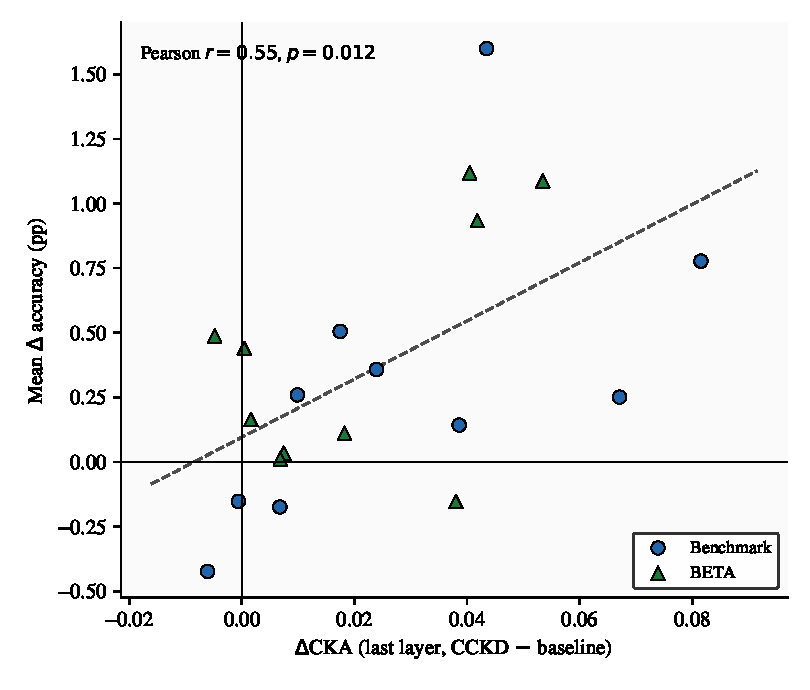
\includegraphics[width=0.62\linewidth]{figures/rq2a_scatter.pdf}
\caption{Last-layer CKA increase induced by CCKD versus accuracy gain, for 20 backbone--dataset--montage settings. Dashed line: linear regression. Circles: Benchmark; triangles: BETA.}
\label{fig:rq2a}
\end{figure}

\subsubsection{Distillation-Layer Intervention Experiment}
\label{sec:layer_intervention}

The correlation above is observational: it does not establish that the CKA increase causes the accuracy gain, since both could instead share a dependence on some other architectural property. As a separate, practical comparison, we vary the set of distillation layers $\mathcal{K} \in \{\texttt{last}, \texttt{mid}, \{\texttt{mid},\texttt{last}\}\}$ to test which layer choice gives the larger accuracy gain, while holding the backbone, dataset, montage, and $\lambda_{sp}$ fixed.

Across the 20 settings, distilling the last layer alone gave a larger gain than distilling the intermediate layer alone in only 5 settings; distilling both layers together matched or exceeded whichever single-layer choice was better in 8 settings. In other words, the main protocol (last-layer distillation \cite{R82}) is not the best choice in most settings: distilling the intermediate layer, alone or combined with the last layer, usually performs as well or better. The per-setting accuracy and $\Delta$CKA at each distilled layer are available in the code repository accompanying this paper (see the Reproducibility section).

\subsection{RQ3: Reliability of Single-Split versus Multi-Split Evaluation}
\label{sec:rq3}

Table~\ref{tab:rq3} compares the conclusion drawn from a single split (2026, Wilcoxon test across subjects) with the conclusion from five splits ($t$-test across splits), for the 20 settings at $\lambda_{sp}=100$ (the RQ1 protocol).

Single-split evaluation misjudges the sign or statistical significance of the effect in 10 of 20 settings: exactly half. The discrepancies go in both directions: a single split can miss a stable improvement or degradation (for example, FB-tCNN Benchmark-3C, DeepConvNet 1C on both datasets), or it can report an effect that does not replicate under multiple splits (for example, ShallowConvNet BETA-3C). The two tests do not share the same unit of replication (Wilcoxon replicates across subjects, the $t$-test replicates across splits), so the table does not indicate which test has higher statistical power. What the table shows is that a study reporting only a single split can reach a conclusion opposite to the one reached when repeating the evaluation on different subject sets. This risk is largest at the effect sizes typical of the SSVEP CCKD literature (under 1--2~pp).

\begin{table}[htbp]
\caption{Conclusion from a single split (2026) versus five splits, $\lambda_{sp}=100$. $+$/$-$/$0$: improves/degrades/not significant ($p<0.05$). $^\star$: conclusions differ (in sign or statistical significance). Student montage: 3C $=\{$O1, Oz, O2$\}$ (3 electrodes), 1C $=\{$Oz$\}$ (1 electrode).}
\label{tab:rq3}
\begin{center}
\footnotesize
\begin{tabular}{llcccc}
\toprule
Backbone & Student & Single split (pp, $p$) & Five splits (pp, $p$) & Benchmark & BETA \\
\midrule
FB-tCNN & 3C & $+0.31$ (0.359) & $+0.78$ (0.0043) & $0 \to +$ $^\star$ & $0 \to +$ $^\star$ \\
 & 1C & $+0.22$ (0.447) & $+0.25$ (0.138) & $0 \to 0$ & $0 \to 0$ \\
DeepConvNet & 3C & $+0.17$ (0.492) & $+0.36$ (0.050) & $0 \to 0$ & $+ \to +$ \\
 & 1C & $+0.01$ (0.980) & $+0.14$ (0.025) & $0 \to +$ $^\star$ & $0 \to 0$ $^\star$ \\
EEGNet & 3C & $-0.20$ (0.770) & $+0.98$ (0.094) & $0 \to 0$ $^\star$ & $- \to -$ \\
 & 1C & $+0.32$ (0.557) & $-0.36$ (0.310) & $0 \to 0$ $^\star$ & $- \to -$ \\
ShallowConvNet & 3C & $-0.52$ (0.322) & $-0.75$ (0.043) & $0 \to -$ $^\star$ & $0 \to 0$ \\
 & 1C & $-0.67$ (0.041) & $-1.01$ (0.011) & $- \to -$ & $+ \to +$ \\
Compact-CNN & 3C & $-0.15$ (0.820) & $+0.18$ (0.646) & $0 \to 0$ $^\star$ & $0 \to 0$ $^\star$ \\
 & 1C & $-0.97$ (0.014) & $-0.43$ (0.124) & $- \to 0$ $^\star$ & $0 \to 0$ \\
\bottomrule
\end{tabular}
\end{center}
\end{table}

\subsection{RQ4: Embedded Deployment}
\label{sec:rq4}

This subsection uses four distinct quantization or fixed-point schemes, one per sub-experiment, because each targets a different property (accuracy preservation, simulated bit-width sensitivity, CPU latency, and FPGA synthesis), and no single scheme satisfied all four tools' constraints. These schemes are not evaluated together as one deployed artifact; each is identified explicitly below. We apply static post-training INT8 quantization (PTQ) to the student models already trained for RQ1, re-evaluating only on the test set without retraining. For the 2 backbone--dataset--montage settings that remained statistically significant after Holm--Bonferroni correction (RQ1, both on EEGNet with BETA, montages 3C and 1C), the accuracy deviation caused by PTQ kept the same sign as FP32 in all 10/10 split--seed settings (100\%) and did not exceed 0.26~pp. This deviation is smaller than the typical split-to-split standard deviation of $\Delta$ across the 20 RQ1 settings (median 0.48~pp, interquartile range 0.31--0.69~pp, computed from the per-setting $sd_{pp}$ values underlying Table~\ref{tab:rq1}).

We further sweep the fixed-point bit width $\{16,12,10,8\}$ using hls4ml's bit-accurate simulation for EEGNet and DeepConvNet on the BETA dataset with 5 splits. These are the smallest and largest backbones by actual parameter count (EEGNet: 5{,}640--5{,}672 parameters; DeepConvNet: 99{,}940--101{,}190 parameters, depending on montage, versus 44{,}488--90{,}536 for the other three backbones). EEGNet's accuracy stays within 1~pp of FP32 at 10 bits or above and drops by more than 4~pp below 8 bits at both montages, matching the 8--10-bit breakpoint range predicted before measurement. DeepConvNet (montage 3C) remains nearly unchanged at 10--16 bits (deviation under 0.05~pp) but drops sharply below 8 bits (deviation of 1.5~pp at 8 bits, 20.4~pp at 6 bits, with an additional sweep around the breakpoint within the range locked in advance). This shows that the true breakpoint lies between 6 and 8 bits, one step lower than the predicted range.

We measure the inference latency of all 5 backbones at FP32 and INT8 on a Raspberry Pi 4 (Cortex-A72) and the Cortex-A53 processing system (PS) of a Xilinx ZCU104. Each setting is averaged over 7 independent processes, 100 inferences per process, batch size 1, 1.0~s window. Here, INT8 uses weight-only dynamic quantization (only the convolution/linear layer weights are quantized; activations remain at FP32). Static quantization raised an incompatibility error with the quantized kernel for the ELU and square operators used in FB-tCNN, DeepConvNet, and ShallowConvNet, confirmed identically on both boards. EEGNet and Compact-CNN also use ELU but combine it with depthwise rather than ordinary spatial convolution and did not hit this error, so ordinary spatial convolution, not the nonlinearity alone, is the more likely distinguishing factor. At INT8 width, all 5 backbones have a forward-pass latency under 16~ms on both boards, including the added filter-bank time for FB-tCNN (maximum total pipeline of 24.5~ms on the ZCU104 PS). This compute-only latency is about 12 times below an illustrative 300~ms control-loop budget that is assumed rather than sourced from a specific wheelchair or speller controller. It also excludes the 1.0~s SSVEP stimulation window that the same protocol requires before this segment becomes available. It therefore bounds only the classifier's own contribution to the control loop's dead time, not the full decision-to-actuation latency. On the ZCU104 PS, board power measured via the on-board INA226 sensor rises from an idle baseline of 11.75~W to 12.32--12.45~W during continuous back-to-back inference, an inference-attributable increase of 0.61--0.76~W across the 5 backbones at both FP32 and INT8. This increase shows no consistent precision-dependent difference. We do not report the corresponding measurement on the Raspberry Pi 4. The stock board exposes no on-board power or current sensor to software (\texttt{vcgencmd pmic\_read\_adc} returns no registered rail on this firmware), so board-level power is reported for the ZCU104 only.

The measured latency ranking (fastest to slowest: ShallowConvNet, EEGNet, DeepConvNet, Compact-CNN, FB-tCNN) is the same on both boards but does not match the ranking predicted from each backbone's maximum temporal kernel (Table~\ref{tab:backbones}) or from the floating-point operation count (FLOPs) measured directly to replace that proxy. Only 2/5 positions match by kernel and 3/5 positions match by FLOPs, both below the majority threshold (4/5) set before measurement; this is a coarse test, given only 5 possible rank positions. The discrepancy is concentrated in the two fastest backbones: EEGNet has the lowest FLOPs (0.87 million FLOPs at montage 3C) due to depthwise/separable convolution but was measured slightly slower than ShallowConvNet (4.03 million FLOPs) on both boards. This shows that at this very small model scale, execution cost on an ARM CPU is not proportional to parameter count, kernel size, or theoretical FLOPs.

We synthesize EEGNet (montage 1C, BETA split 2026/seed 2026, CCKD student $\lambda_{sp}=100$, 10-bit width) onto the ZCU104's PL (programmable logic, the FPGA fabric). This configuration is one of the two settings (EEGNet, BETA, montages 3C and 1C) where CCKD significantly degraded accuracy after Holm--Bonferroni correction (RQ1, Table~\ref{tab:rq1}). It is evaluated here at a single split and seed (2026/2026) rather than averaged over the five splits used elsewhere in this paper. The hardware test below therefore checks whether the on-board implementation reproduces its own bit-accurate simulation faithfully, not whether CCKD helped at this setting. An initial attempt used \texttt{hls4ml}, a tool that translates a trained network into a bit-accurate fixed-point hardware description for simulation and synthesis, through its VivadoAccelerator backend (AXI-Stream and AXI DMA, a streaming data-transfer interface with its own framing and handshake signals). This attempt reached a working synthesis and bitstream, but a persistent fault in TLAST (the signal marking the last word of a data transfer) on the output stream blocked on-board use; the fault survived six rounds of fixes to that backend. We therefore wrap the same already-verified inference kernel in a hand-written AXI memory-mapped (m\_axi) interface with an AXI-Lite control register, a simpler register-mapped interface that avoids the AXI-Stream framing issue entirely. Vitis HLS and Vivado 2024.2 synthesis, implementation (place and route), and bitstream generation all succeed at a 100~MHz clock, with timing closing at a 2.074~ns margin. Whole-design resource usage (the Zynq processing system and the inference IP) uses 11.75\% of look-up tables (LUT), 6.54\% of flip-flops (FF), and 9.13\% of Block RAM tiles of the XCZU7EV board, with no digital signal processing (DSP) blocks used. This resource usage is far below the 70\% threshold fixed in advance (Section~\ref{sec:setup}). End-to-end latency is 1.17~ms per window, measured as total wall-clock time over 3200 back-to-back inferences divided by window count, including AXI-Lite register writes, the host-side completion-flag polling loop, and PYNQ data marshaling, not only the FPGA's internal compute cycles. We deploy this bitstream to the ZCU104 and run inference on the full 3200-window BETA test set for this setting. On-board accuracy is 24.06\%, versus 24.09\% for the H2 bit-accurate simulation at the same 10-bit width, a difference of 0.03~pp, well within the 1~pp threshold fixed in advance (Section~\ref{sec:setup}). For context, this setting's own non-distilled baseline accuracy is 25.35\%, near the low end of the 22.50--55.83\% range of baseline accuracies across all 20 backbone--dataset--montage settings in this paper. This low baseline is consistent with CCKD's degrading effect here (RQ1). Board power during continuous inference (10.45--10.50~W) does not measurably exceed the idle baseline (10.55~W) at the resolution of the on-board INA226 sensor, consistent with the low utilization of this PL design.

\section{Conclusion}

CCKD does not provide a consistent benefit when extended from FB-tCNN to four other backbones. Of the 20 backbone--dataset--montage settings evaluated at a fixed cross-backbone weight, only 2 remained statistically significant after correction for multiple comparisons, and both were degradations; neither survives at that backbone's own validation-tuned weight, so no setting in this study shows an effect that is both corrected-significant and robust to distillation-weight choice (RQ1). The benefit of CCKD, when present, is sensitive to the specific montage chosen, not only to electrode count (RQ1b). The CKA increase caused by distillation correlates with the accuracy gain across backbones, but this correlation is observational, and the CKA gap before distillation does not predict the gain. Across the three choices of distillation layer tested, distilling the intermediate layer, alone or combined with the last layer, usually outperforms the last-layer distillation protocol \cite{R82} (RQ2). Evaluation on a single subject split, the protocol common in the EEG knowledge-distillation literature, misjudges the sign or statistical significance of the effect in half of the settings (RQ3). The CCKD student model's accuracy effect keeps its sign after INT8 quantization at the two settings that remained statistically significant, both of which were degradations, and tolerates fixed-point quantization down to 8--10 bits for the two backbones tested (EEGNet and DeepConvNet). Every backbone achieves compute-only inference latency far below an illustrative, unsourced wheelchair control-loop budget, even at the lowest arithmetic width measured and excluding the SSVEP stimulation window itself. However, the measured latency does not rank by maximum temporal kernel or by FLOPs for most backbones, so selecting a backbone for a specific embedded platform requires direct measurement rather than inference from the architecture (RQ4). The smallest backbone (EEGNet) synthesizes onto the ZCU104's PL within the board's resource budget (under 12\% LUT, 7\% FF, 10\% BRAM, no DSP used), with timing closed and an end-to-end latency of 1.17~ms per inference. Its on-board accuracy matches the H2 bit-accurate simulation within 0.03~pp, well inside the 1~pp threshold, at the one setting tested. This setting is one where CCKD itself significantly degraded accuracy, so the result validates hardware-simulation fidelity rather than a CCKD accuracy benefit. Overall, these results show that cross-montage relational distillation is backbone- and electrode-position-dependent, and that the sub-1--2-pp gains typical of this literature need to be evaluated over multiple subject splits with statistical correction, rather than stopping at a single split. In practice, this suggests using the validation-split $\Delta$CKA as an inexpensive pre-deployment screen for whether CCKD is likely to help a given backbone-montage pair. The sign of the effect should still be confirmed on held-out subjects before relying on it in a wheelchair, speller, or robotic-arm control loop, rather than assuming the benefit reported for one backbone on one split in prior work.

\noindent \textbf{Reproducibility.} The training, preprocessing, and statistical-analysis code, the per-split subject-assignment lists, the seeds, and the per-run results are publicly available at \url{https://github.com/nguyenphuonghuy/SSVEP_CCKD}. The software environment is version-pinned. Because GPU training is not bit-exact reproducible, repeated runs vary within the range measured in Section~\ref{sec:rq3} (RQ3).
\\
\\
\noindent \textbf{Author Contribution:} All authors contributed equally to this paper. All authors read and approved the final manuscript.

\noindent \textbf{Funding:} This research received no external funding.

\noindent \textbf{Acknowledgment:} This work was carried out in part at the Thai Nguyen University of Technology, and at the Northern, Central and Southern Region Shared Key Laboratory, specializing in the fields of Internet of Things (IoT), High-Performance Computing (HPC) and Unmanned Aerial Vehicles (UAVs), Viet Nam.

\noindent \textbf{Conflicts of Interest:} The authors declare no conflict of interest.

\section*{References}
\small{
\begin{thebibliography}{99}
\itemsep 0pt
\bibitem{R3} W. Chen, S. Chen, Y. Liu, Y. Chen, and C. Chen, "An Electric Wheelchair Manipulating System Using SSVEP-Based BCI System," \textit{Biosensors}, vol. 12, no. 10, pp. 772, Sep. 2022, \url{https://doi.org/10.3390/bios12100772}.

\bibitem{R6} V. Sakkalis, M. Krana, C. Farmaki, C. Bourazanis, D. Gaitatzis, and M. Pediaditis, "Augmented Reality Driven Steady-State Visual Evoked Potentials for Wheelchair Navigation," \textit{IEEE Transactions on Neural Systems and Rehabilitation Engineering}, vol. 30, pp. 2960-2969, Nov. 2022, \url{https://doi.org/10.1109/TNSRE.2022.3215695}.

\bibitem{R7} K. Liu, Y. Yu, Y. Liu, J. Tang, X. Liang, X. Chu, and Z. Zhou, "A novel brain-controlled wheelchair combined with computer vision and augmented reality," \textit{BioMedical Engineering OnLine}, vol. 21, no. 1, Dec. 2022, \url{https://doi.org/10.1186/s12938-022-01020-8}.

\bibitem{R8} H. Rivera-Flor, D. Gurve, A. Floriano, D. Delisle-Rodriguez, R. Mello, and T. Bastos-Filho, "CCA-Based Compressive Sensing for SSVEP-Based Brain-Computer Interfaces to Command a Robotic Wheelchair," \textit{IEEE Transactions on Instrumentation and Measurement}, vol. 71, pp. 1-10, Nov. 2022, \url{https://doi.org/10.1109/TIM.2022.3218102}.

\bibitem{R9} M. Albán-Escobar, P. Navarrete-Arroyo, D. R. D. l. Cruz-Guevara, and J. Tobar-Quevedo, "Assistance Device Based on SSVEP-BCI Online to Control a 6-DOF Robotic Arm," \textit{Sensors}, vol. 24, no. 6, pp. 1922, Mar. 2024, \url{https://doi.org/10.3390/s24061922}.

\bibitem{R4} X. Bai, M. Li, S. Qi, A. C. M. Ng, T. Ng, and W. Qian, "A hybrid P300-SSVEP brain-computer interface speller with a frequency enhanced row and column paradigm," \textit{Frontiers in Neuroscience}, vol. 17, Mar. 2023, \url{https://doi.org/10.3389/fnins.2023.1133933}.

\bibitem{R5} S. Wang, B. Ji, D. Shao, W. Chen, and K. Gao, "A Methodology for Enhancing SSVEP Features Using Adaptive Filtering Based on the Spatial Distribution of EEG Signals," \textit{Micromachines}, vol. 14, no. 5, pp. 976, Apr. 2023, \url{https://doi.org/10.3390/mi14050976}.

\bibitem{R39} S. Liu, D. Zhang, Z. Liu, M. Liu, Z. Ming, T. Liu, D. Suo, S. Funahashi, and T. Yan, "Review of brain–computer interface based on steady‐state visual evoked potential," \textit{Brain Science Advances}, vol. 8, no. 4, pp. 258-275, Dec. 2022, \url{https://doi.org/10.26599/BSA.2022.9050022}.

\bibitem{R40} A. S. Albahri, Z. T. Al-qaysi, L. Alzubaidi, A. Alnoor, O. S. Albahri, A. H. Alamoodi, and A. A. Bakar, "A Systematic Review of Using Deep Learning Technology in the Steady-State Visually Evoked Potential-Based Brain-Computer Interface Applications: Current Trends and Future Trust Methodology," \textit{International Journal of Telemedicine and Applications}, vol. 2023, pp. 1-24, Apr. 2023, \url{https://doi.org/10.1155/2023/7741735}.

\bibitem{R41} Z. T. Al-Qaysi, A. S. Albahri, M. A. Ahmed, R. A. Hamid, M. A. Alsalem, O. S. Albahri, A. H. Alamoodi, R. Z. Homod, G. G. Shayea, and A. M. Duhaim, "A comprehensive review of deep learning power in steady-state visual evoked potentials," \textit{Neural Computing and Applications}, vol. 36, no. 27, pp. 16683-16706, Sep. 2024, \url{https://doi.org/10.1007/s00521-024-10143-z}.

\bibitem{R36} H. Kim, and C. Im, "Influence of the Number of Channels and Classification Algorithm on the Performance Robustness to Electrode Shift in Steady-State Visual Evoked Potential-Based Brain-Computer Interfaces," \textit{Frontiers in Neuroinformatics}, vol. 15, Oct. 2021, \url{https://doi.org/10.3389/fninf.2021.750839}.

\bibitem{R38} H. Zhao, L. Zheng, M. Yuan, Y. Wang, X. Gao, R. Liu, and W. Pei, "Optimization of ear electrodes for SSVEP-based BCI," \textit{Journal of Neural Engineering}, vol. 20, no. 4, pp. 046011, Aug. 2023, \url{https://doi.org/10.1088/1741-2552/acdf85}.

\bibitem{R47} X. Huang, S. Chen, and C. Wei, "Enhancing Low-Density EEG-Based Brain-Computer Interfacing With Similarity-Keeping Knowledge Distillation," \textit{IEEE Transactions on Emerging Topics in Computational Intelligence}, vol. 8, no. 2, pp. 1156-1166, Apr. 2024, \url{https://doi.org/10.1109/TETCI.2023.3335943}.

\bibitem{R82} D. M. Thuong, and N. P. Huy, "Cross-Channel Relational Knowledge Distillation for Low-Electrode SSVEP Recognition," in \textit{Proc. International Conference on Advanced Engineering and Robotics Applications (ICERA)}, Paper no. 271, 2026, accepted, in press.

\bibitem{R16} W. Ding, J. Shan, B. Fang, C. Wang, F. Sun, and X. Li, "Filter Bank Convolutional Neural Network for Short Time-Window Steady-State Visual Evoked Potential Classification," \textit{IEEE Transactions on Neural Systems and Rehabilitation Engineering}, vol. 29, pp. 2615-2624, Dec. 2021, \url{https://doi.org/10.1109/TNSRE.2021.3132162}.

\bibitem{R48} Y. Zheng, S. Wu, J. Chen, Q. Yao, and S. Zheng, "Cross-Subject Motor Imagery Electroencephalogram Decoding with Domain Generalization," \textit{Bioengineering}, vol. 12, no. 5, pp. 495, May 2025, \url{https://doi.org/10.3390/bioengineering12050495}.

\bibitem{R49} Z. Xu, and Z. Yu, "Entropy-Based Dual-Teacher Distillation for Efficient Motor Imagery EEG Classification," \textit{Entropy}, vol. 28, no. 3, pp. 310, Mar. 2026, \url{https://doi.org/10.3390/e28030310}.

\bibitem{R50} Z. Zhang, and G. Lu, "Multimodal Knowledge Distillation for Emotion Recognition," \textit{Brain Sciences}, vol. 15, no. 7, pp. 707, Jun. 2025, \url{https://doi.org/10.3390/brainsci15070707}.

\bibitem{R51} S. Zhang, C. Tang, and C. Guan, "Visual-to-EEG cross-modal knowledge distillation for continuous emotion recognition," \textit{Pattern Recognition}, vol. 130, pp. 108833, Oct. 2022, \url{https://doi.org/10.1016/j.patcog.2022.108833}.

\bibitem{R52} C. Cheng, W. Liu, X. Wang, L. Feng, and Z. Jia, "DISD-Net: A Dynamic Interactive Network With Self-Distillation for Cross-Subject Multi-Modal Emotion Recognition," \textit{IEEE Transactions on Multimedia}, vol. 27, pp. 4643-4655, Jan. 2025, \url{https://doi.org/10.1109/TMM.2025.3535344}.

\bibitem{R53} J. Wu, B. Tang, Y. Wang, C. Li, and Q. Yang, "A multi-level teacher assistant-based knowledge distillation framework with dynamic feedback for motor imagery EEG decoding," \textit{Neural Networks}, vol. 194, pp. 108180, Feb. 2026, \url{https://doi.org/10.1016/j.neunet.2025.108180}.

\bibitem{R15} J. Chen, Y. Zhang, Y. Pan, P. Xu, and C. Guan, "A transformer-based deep neural network model for SSVEP classification," \textit{Neural Networks}, vol. 164, pp. 521-534, Jul. 2023, \url{https://doi.org/10.1016/j.neunet.2023.04.045}.

\bibitem{R23} Y. HUANG, Y. CHEN, L. CAO, Y. CAO, X. YANG, Y. DONG, and T. LIU, "INCEPFORMERNET: A MULTI-SCALE MULTI-HEAD ATTENTION NETWORK FOR SSVEP CLASSIFICATION," \textit{Journal of Mechanics in Medicine and Biology}, vol. 25, no. 08, Oct. 2025, \url{https://doi.org/10.1142/S0219519425400809}.

\bibitem{R18} S. Zhang, D. An, J. Liu, J. Chen, Y. Wei, and F. Sun, "Dynamic decomposition graph convolutional neural network for SSVEP-based brain–computer interface," \textit{Neural Networks}, vol. 172, pp. 106075, Apr. 2024, \url{https://doi.org/10.1016/j.neunet.2023.12.029}.

\bibitem{R19} Y. Pan, J. Chen, Y. Zhang, and Y. Zhang, "An efficient CNN-LSTM network with spectral normalization and label smoothing technologies for SSVEP frequency recognition," \textit{Journal of Neural Engineering}, vol. 19, no. 5, pp. 056014, Oct. 2022, \url{https://doi.org/10.1088/1741-2552/ac8dc5}.

\bibitem{R20} Z. Wang, C. M. Wong, B. Wang, Z. Feng, F. Cong, and F. Wan, "Compact Artificial Neural Network Based on Task Attention for Individual SSVEP Recognition With Less Calibration," \textit{IEEE Transactions on Neural Systems and Rehabilitation Engineering}, vol. 31, pp. 2525-2534, May 2023, \url{https://doi.org/10.1109/TNSRE.2023.3276745}.

\bibitem{R21} S. Huang, and Q. Wei, "A deep learning model combining convolutional neural networks and a selective kernel mechanism for SSVEP-Based BCIs," \textit{Computers in Biology and Medicine}, vol. 196, pp. 110691, Sep. 2025, \url{https://doi.org/10.1016/j.compbiomed.2025.110691}.

\bibitem{R26} R. Ma, Y. Cao, S. Q. Xie, M. Zhang, J. Li, and Z. Zhang, "LGFCNN: A synergistic framework integrating graph-based spatial filter and lightweight CNN for SSVEP recognition," \textit{Neurocomputing}, vol. 656, pp. 131561, Dec. 2025, \url{https://doi.org/10.1016/j.neucom.2025.131561}.

\bibitem{R29} V. P. Oikonomou, "MultiHeadEEGModelCLS: Contextual Alignment and Spatio-Temporal Attention Model for EEG-Based SSVEP Classification," \textit{Electronics}, vol. 14, no. 22, pp. 4394, Nov. 2025, \url{https://doi.org/10.3390/electronics14224394}.

\bibitem{R75} J. White, and S. D. Power, "k-Fold Cross-Validation Can Significantly Over-Estimate True Classification Accuracy in Common EEG-Based Passive BCI Experimental Designs: An Empirical Investigation," \textit{Sensors}, vol. 23, no. 13, pp. 6077, Jul. 2023, \url{https://doi.org/10.3390/s23136077}.

\bibitem{R76} F. D. Pup, A. Zanola, L. F. Tshimanga, A. Bertoldo, L. Finos, and M. Atzori, "The role of data partitioning on the performance of EEG-based deep learning models in supervised cross-subject analysis: A preliminary study," \textit{Computers in Biology and Medicine}, vol. 196, pp. 110608, Sep. 2025, \url{https://doi.org/10.1016/j.compbiomed.2025.110608}.

\bibitem{R77} G. Brookshire, J. Kasper, N. M. Blauch, Y. C. Wu, R. Glatt, D. A. Merrill, S. Gerrol, K. J. Yoder, C. Quirk, and C. Lucero, "Data leakage in deep learning studies of translational EEG," \textit{Frontiers in Neuroscience}, vol. 18, May 2024, \url{https://doi.org/10.3389/fnins.2024.1373515}.

\bibitem{R78} H. Lee, H. Cheon, S. Lee, M. Shim, and H. Hwang, "Risk of data leakage in estimating the diagnostic performance of a deep-learning-based computer-aided system for psychiatric disorders," \textit{Scientific Reports}, vol. 13, no. 1, Oct. 2023, \url{https://doi.org/10.1038/s41598-023-43542-8}.

\bibitem{R79} A. Kamrud, B. Borghetti, and C. S. Kabban, "The Effects of Individual Differences, Non-Stationarity, and the Importance of Data Partitioning Decisions for Training and Testing of EEG Cross-Participant Models," \textit{Sensors}, vol. 21, no. 9, pp. 3225, May 2021, \url{https://doi.org/10.3390/s21093225}.

\bibitem{R80} L. Xu, M. Xu, Y. Ke, X. An, S. Liu, and D. Ming, "Cross-Dataset Variability Problem in EEG Decoding With Deep Learning," \textit{Frontiers in Human Neuroscience}, vol. 14, Apr. 2020, \url{https://doi.org/10.3389/fnhum.2020.00103}.

\bibitem{R81} M. Geethapriya, and K. Pattabiraman, "Subject-independent classification of ADHD from pediatric EEG: a leakage-aware deep learning framework with interpretable neurophysiological mapping," \textit{Frontiers in Neuroscience}, vol. 20, Oct. 2026, \url{https://doi.org/10.3389/fnins.2026.1925266}.

\bibitem{R73} S. Kornblith, M. Norouzi, H. Lee, and G. Hinton, "Similarity of Neural Network Representations Revisited," in \textit{Proceedings of the 36th International Conference on Machine Learning (ICML 2019)}, PMLR 97, pp. 3519-3529, 2019, \url{https://proceedings.mlr.press/v97/kornblith19a.html}.
\bibitem{R74} C. Cortes, M. Mohri, and A. Rostamizadeh, "Algorithms for Learning Kernels Based on Centered Alignment," \textit{Journal of Machine Learning Research}, vol. 13, pp. 795-828, 2012, \url{https://jmlr.org/papers/v13/cortes12a.html}.
\bibitem{R71} S. A. Alvarez, "Gaussian RBF Centered Kernel Alignment (CKA) in the Large-Bandwidth Limit," \textit{IEEE Transactions on Pattern Analysis and Machine Intelligence}, vol. 45, no. 5, pp. 6587-6593, May 2023, \url{https://doi.org/10.1109/TPAMI.2022.3216518}.

\bibitem{R72} N. Kriegeskorte, and X. Wei, "Neural tuning and representational geometry," \textit{Nature Reviews Neuroscience}, vol. 22, no. 11, pp. 703-718, Nov. 2021, \url{https://doi.org/10.1038/s41583-021-00502-3}.

\bibitem{R70} M. Tobón-Henao, A. M. Álvarez-Meza, and C. G. Castellanos-Dominguez, "Kernel-Based Regularized EEGNet Using Centered Alignment and Gaussian Connectivity for Motor Imagery Discrimination," \textit{Computers}, vol. 12, no. 7, pp. 145, Jul. 2023, \url{https://doi.org/10.3390/computers12070145}.

\bibitem{R58} Y. Xie, and S. Oniga, "A Comprehensive Review of Hardware Acceleration Techniques and Convolutional Neural Networks for EEG Signals," \textit{Sensors}, vol. 24, no. 17, pp. 5813, Sep. 2024, \url{https://doi.org/10.3390/s24175813}.

\bibitem{R60} F. Pacini, T. Pacini, G. Lai, A. M. Zocco, and L. Fanucci, "Design and Evaluation of CPU-, GPU-, and FPGA-Based Deployment of a CNN for Motor Imagery Classification in Brain-Computer Interfaces," \textit{Electronics}, vol. 13, no. 9, pp. 1646, Apr. 2024, \url{https://doi.org/10.3390/electronics13091646}.

\bibitem{R62} A. Palumbo, N. Ielpo, and B. Calabrese, "An FPGA-Embedded Brain-Computer Interface System to Support Individual Autonomy in Locked-In Individuals," \textit{Sensors}, vol. 22, no. 1, pp. 318, Jan. 2022, \url{https://doi.org/10.3390/s22010318}.

\bibitem{R63} P. Novac, G. B. Hacene, A. Pegatoquet, B. Miramond, and V. Gripon, "Quantization and Deployment of Deep Neural Networks on Microcontrollers," \textit{Sensors}, vol. 21, no. 9, pp. 2984, Apr. 2021, \url{https://doi.org/10.3390/s21092984}.

\bibitem{R17} Y. Li, J. Xiang, and T. Kesavadas, "Convolutional Correlation Analysis for Enhancing the Performance of SSVEP-Based Brain-Computer Interface," \textit{IEEE Transactions on Neural Systems and Rehabilitation Engineering}, vol. 28, no. 12, pp. 2681-2690, Dec. 2020, \url{https://doi.org/10.1109/TNSRE.2020.3038718}.

\bibitem{R22} P. Israsena, and S. Pan-Ngum, "A CNN-Based Deep Learning Approach for SSVEP Detection Targeting Binaural Ear-EEG," \textit{Frontiers in Computational Neuroscience}, vol. 16, May 2022, \url{https://doi.org/10.3389/fncom.2022.868642}.

\bibitem{R25} X. Li, S. Yang, N. Fei, J. Wang, W. Huang, and Y. Hu, "A Convolutional Neural Network for SSVEP Identification by Using a Few-Channel EEG," \textit{Bioengineering}, vol. 11, no. 6, pp. 613, Jun. 2024, \url{https://doi.org/10.3390/bioengineering11060613}.

\bibitem{R37} A. Kiser, A. Cantürk, and I. Volosyak, "SSVEP-driven BCI authentication with reduced number of EEG electrodes across high and low frequency ranges," \textit{Frontiers in Neuroergonomics}, vol. 7, Mar. 2026, \url{https://doi.org/10.3389/fnrgo.2026.1741655}.

\bibitem{R54} Y. Zhang, H. Liu, Y. Xiao, M. Amoon, D. Zhang, D. Wang, S. Yang, and C. Quek, "LLM-Enhanced Multi-Teacher Knowledge Distillation for Modality-Incomplete Emotion Recognition in Daily Healthcare," \textit{IEEE Journal of Biomedical and Health Informatics}, vol. 29, no. 9, pp. 6406-6416, Sep. 2025, \url{https://doi.org/10.1109/JBHI.2024.3470338}.

\bibitem{R55} Y. Zhang, W. Chen, X. Cai, and C. Cheng, "SASD-MCL: Semi-supervised alignment self-distillation with mixed contrastive learning for cross-subject EEG emotion recognition," \textit{Neural Networks}, vol. 190, pp. 107614, Oct. 2025, \url{https://doi.org/10.1016/j.neunet.2025.107614}.

\bibitem{R57} W. Li, S. Wang, S. Shao, and K. Huang, "Distillation-Based Domain Generalization for Cross-Dataset EEG-Based Emotion Recognition," \textit{IEEE Transactions on Emerging Topics in Computational Intelligence}, vol. 9, no. 3, pp. 2474-2490, Jun. 2025, \url{https://doi.org/10.1109/TETCI.2024.3449926}.

\bibitem{R56} S. Zhong, J. Shi, and Y. Wang, "Knowledge-guided quantization-aware training for EEG-based emotion recognition," \textit{Journal of Visual Communication and Image Representation}, vol. 108, pp. 104415, Apr. 2025, \url{https://doi.org/10.1016/j.jvcir.2025.104415}.

\bibitem{R2} X. Mai, J. Ai, M. Ji, X. Zhu, and J. Meng, "A hybrid BCI combining SSVEP and EOG and its application for continuous wheelchair control," \textit{Biomedical Signal Processing and Control}, vol. 88, pp. 105530, Feb. 2024, \url{https://doi.org/10.1016/j.bspc.2023.105530}.

\bibitem{R10} M. Y. M. Naser, and S. Bhattacharya, "Towards Practical BCI-Driven Wheelchairs: A Systematic Review Study," \textit{IEEE Transactions on Neural Systems and Rehabilitation Engineering}, vol. 31, pp. 1030-1044, Jan. 2023, \url{https://doi.org/10.1109/tnsre.2023.3236251}.

\bibitem{R11} U. F. Ukaegbu, S. Houshmand, L. Hammond, K. Adams, J. Andersen, and H. Rouhani, "Navigation paradigms for non-invasive BCI-controlled wheelchairs: a systematic review," \textit{Progress in Biomedical Engineering}, vol. 8, no. 2, pp. 022008, Jun. 2026, \url{https://doi.org/10.1088/2516-1091/ae5563}.

\bibitem{R64} H. Chu, Y. Yan, L. Gan, H. Jia, L. Qian, Y. Huan, L. Zheng, and Z. Zou, "A Neuromorphic Processing System With Spike-Driven SNN Processor for Wearable ECG Classification," \textit{IEEE Transactions on Biomedical Circuits and Systems}, vol. 16, no. 4, pp. 511-523, Aug. 2022, \url{https://doi.org/10.1109/TBCAS.2022.3189364}.

\bibitem{R65} S. Zhao, J. Yang, J. Wang, C. Fang, T. Liu, S. Zhang, and M. Sawan, "A 0.99-to-4.38 uJ/class Event-Driven Hybrid Neural Network Processor for Full-Spectrum Neural Signal Analyses," \textit{IEEE Transactions on Biomedical Circuits and Systems}, vol. 17, no. 3, pp. 598-609, Jun. 2023, \url{https://doi.org/10.1109/TBCAS.2023.3268502}.

\bibitem{R66} P. Busia, G. Leone, A. Matticola, L. Raffo, and P. Meloni, "Wearable Epilepsy Seizure Detection on FPGA With Spiking Neural Networks," \textit{IEEE Transactions on Biomedical Circuits and Systems}, vol. 19, no. 6, pp. 1175-1186, Dec. 2025, \url{https://doi.org/10.1109/TBCAS.2025.3575327}.

\bibitem{R67} M. A. Scrugli, G. Leone, P. Busia, L. Raffo, and P. Meloni, "All-Spiking ECG Analysis for Arrhythmia Classification on Low-Power FPGA," \textit{IEEE Sensors Journal}, vol. 26, no. 7, pp. 11372-11386, Apr. 2026, \url{https://doi.org/10.1109/JSEN.2026.3663715}.

\bibitem{R68} L. Yuan, J. Wei, and Y. Liu, "Spiking neural networks for EEG signal analysis using wavelet transform," \textit{Frontiers in Neuroscience}, vol. 19, Oct. 2025, \url{https://doi.org/10.3389/fnins.2025.1652274}.

\bibitem{R69} A. R. Aslam, and M. A. B. Altaf, "An On-Chip Processor for Chronic Neurological Disorders Assistance Using Negative Affectivity Classification," \textit{IEEE Transactions on Biomedical Circuits and Systems}, vol. 14, no. 4, pp. 838-851, Aug. 2020, \url{https://doi.org/10.1109/TBCAS.2020.3008766}.

\bibitem{R61} M. Nguyen, T. Do, X. Tran, Q. Nguyen, and C. Lin, "Edge AI-Brain–Computer Interfaces System: A Survey," \textit{IEEE Transactions on Neural Systems and Rehabilitation Engineering}, vol. 33, pp. 4051-4066, Oct. 2025, \url{https://doi.org/10.1109/TNSRE.2025.3618688}.

\bibitem{R83} R. T. Schirrmeister, J. T. Springenberg, L. D. J. Fiederer, M. Glasstetter, K. Eggensperger, M. Tangermann, F. Hutter, W. Burgard, and T. Ball, "Deep learning with convolutional neural networks for EEG decoding and visualization," \textit{Human Brain Mapping}, vol. 38, no. 11, pp. 5391-5420, Nov. 2017, \url{https://doi.org/10.1002/hbm.23730}.

\bibitem{R84} V. J. Lawhern, A. J. Solon, N. R. Waytowich, S. M. Gordon, C. P. Hung, and B. J. Lance, "EEGNet: a compact convolutional neural network for EEG-based brain-computer interfaces," \textit{Journal of Neural Engineering}, vol. 15, no. 5, pp. 056013, Oct. 2018, \url{https://doi.org/10.1088/1741-2552/aace8c}.

\bibitem{R85} N. Waytowich, V. J. Lawhern, J. O. Garcia, J. Cummings, J. Faller, P. Sajda, and J. M. Vettel, "Compact convolutional neural networks for classification of asynchronous steady-state visual evoked potentials," \textit{Journal of Neural Engineering}, vol. 15, no. 6, pp. 066031, Dec. 2018, \url{https://doi.org/10.1088/1741-2552/aae5d8}.

\bibitem{R86} S. Holm, "A simple sequentially rejective multiple test procedure," \textit{Scandinavian Journal of Statistics}, vol. 6, no. 2, pp. 65-70, 1979, \url{https://www.jstor.org/stable/4615733}.

\bibitem{R1} A. M. A. Ahmed, Y. Al-Junaidi, A. Al-Tayar, A. Qaid, and K. K. Qureshi, "An SSVEP-Based Brain–Computer Interface Device for Wheelchair Control Integrated with a Speech Aid System," \textit{Eng}, vol. 6, no. 12, pp. 343, Dec. 2025, \url{https://doi.org/10.3390/eng6120343}.

\bibitem{R12} X. He, I. Daly, W. Gu, Y. Chen, X. Wu, W. Chen, X. Wang, A. Cichocki, and J. Jin, "TBMSCCN: Two-Branch Multi-Scale Convolutional Correlation Network for Steady-State Visual Evoked Potential Classification," \textit{IEEE Transactions on Biomedical Engineering}, pp. 1-16, Mar. 2026, \url{https://doi.org/10.1109/TBME.2026.3676014}.

\bibitem{R13} Z. Lan, Z. Li, C. Yan, X. Xiang, D. Tang, M. Wu, and Z. Chen, "MTSNet: Convolution-Based Transformer Network With Multi-Scale Temporal-Spectral Feature Fusion for SSVEP Signal Decoding," \textit{IEEE Journal of Biomedical and Health Informatics}, vol. 29, no. 11, pp. 8034-8047, Nov. 2025, \url{https://doi.org/10.1109/JBHI.2025.3573410}.

\bibitem{R14} Y. Song, Q. Zheng, B. Liu, and X. Gao, "EEG Conformer: Convolutional Transformer for EEG Decoding and Visualization," \textit{IEEE Transactions on Neural Systems and Rehabilitation Engineering}, vol. 31, pp. 710-719, Dec. 2023, \url{https://doi.org/10.1109/TNSRE.2022.3230250}.

\bibitem{R24} Q. Wei, C. Li, Y. Wang, and X. Gao, "Enhancing the performance of SSVEP-based BCIs by combining task-related component analysis and deep neural network," \textit{Scientific Reports}, vol. 15, no. 1, Jan. 2025, \url{https://doi.org/10.1038/s41598-024-84534-6}.

\bibitem{R27} S. Shen, Y. Ke, and D. Ming, "Enhancing SSVEP recognition for short data via time series forecasting," \textit{Expert Systems with Applications}, vol. 303, pp. 130640, Mar. 2026, \url{https://doi.org/10.1016/j.eswa.2025.130640}.

\bibitem{R28} Z. Ji, T. Xu, C. Chen, H. Yin, F. Wan, and H. Wang, "Subject-specific CNN model with parameter-based transfer learning for SSVEP detection," \textit{Biomedical Signal Processing and Control}, vol. 103, pp. 107404, May 2025, \url{https://doi.org/10.1016/j.bspc.2024.107404}.

\bibitem{R30} X. Wen, S. Jia, D. Han, Y. Dong, C. Gao, R. Cao, Y. Hao, Y. Guo, and R. Cao, "Filter banks guided correlational convolutional neural network for SSVEPs based BCI classification," \textit{Journal of Neural Engineering}, vol. 21, no. 5, pp. 056024, Oct. 2024, \url{https://doi.org/10.1088/1741-2552/ad7f89}.

\bibitem{R31} H. Xiong, J. Song, J. Liu, and Y. Han, "Deep transfer learning-based SSVEP frequency domain decoding method," \textit{Biomedical Signal Processing and Control}, vol. 89, pp. 105931, Mar. 2024, \url{https://doi.org/10.1016/j.bspc.2023.105931}.

\bibitem{R32} J. Yang, S. Zhao, W. Zhang, and X. Liu, "High-Order Temporal Convolutional Network for Improving Classification Performance of SSVEP-EEG," \textit{IRBM}, vol. 45, no. 2, pp. 100830, Apr. 2024, \url{https://doi.org/10.1016/j.irbm.2024.100830}.

\bibitem{R33} G. Xia, L. Wang, S. Xiong, and J. Deng, "Enhancing detection of SSVEP-based BCIs via a novel temporally local canonical correlation analysis," \textit{Journal of Neuroscience Methods}, vol. 414, pp. 110325, Feb. 2025, \url{https://doi.org/10.1016/j.jneumeth.2024.110325}.

\bibitem{R34} S. Hamou, M. Moufassih, O. Tarahi, S. Agounad, and H. I. Azami, "Hybrid approach: combining eCCA and SSCOR for enhancing SSVEP decoding," \textit{The Journal of Supercomputing}, vol. 80, no. 10, pp. 14391-14416, Jul. 2024, \url{https://doi.org/10.1007/s11227-024-06027-7}.

\bibitem{R35} K. Hu, Y. Wang, K. Tu, H. Guo, and J. Yan, "Cross-domain correlation analysis to improve SSVEP signals recognition in brain-computer interfaces," \textit{Biomedical Physics \& Engineering Express}, vol. 12, no. 1, pp. 015021, Feb. 2026, \url{https://doi.org/10.1088/2057-1976/ae2772}.

\bibitem{R42} C. Reitelbach, and K. Oyibo, "Optimal Stimulus Properties for Steady-State Visually Evoked Potential Brain–Computer Interfaces: A Scoping Review," \textit{Multimodal Technologies and Interaction}, vol. 8, no. 2, pp. 6, Jan. 2024, \url{https://doi.org/10.3390/mti8020006}.

\bibitem{R43} A. Kawala-Sterniuk, N. Browarska, A. Al-Bakri, M. Pelc, J. Zygarlicki, M. Sidikova, R. Martinek, and E. J. Gorzelanczyk, "Summary of over Fifty Years with Brain-Computer Interfaces—A Review," \textit{Brain Sciences}, vol. 11, no. 1, pp. 43, Jan. 2021, \url{https://doi.org/10.3390/brainsci11010043}.

\bibitem{R44} X. Zhang, L. Yao, X. Wang, J. Monaghan, D. McAlpine, and Y. Zhang, "A survey on deep learning-based non-invasive brain signals: recent advances and new frontiers," \textit{Journal of Neural Engineering}, vol. 18, no. 3, pp. 031002, Jun. 2021, \url{https://doi.org/10.1088/1741-2552/abc902}.

\bibitem{R45} B. Abibullaev, A. Keutayeva, and A. Zollanvari, "Deep Learning in EEG-Based BCIs: A Comprehensive Review of Transformer Models, Advantages, Challenges, and Applications," \textit{IEEE Access}, vol. 11, pp. 127271-127301, Nov. 2023, \url{https://doi.org/10.1109/access.2023.3329678}.

\bibitem{R46} E. Karikari, and K. A. Koshechkin, "Review on brain-computer interface technologies in healthcare," \textit{Biophysical Reviews}, vol. 15, no. 5, pp. 1351-1358, Oct. 2023, \url{https://doi.org/10.1007/s12551-023-01138-6}.

\bibitem{R59} B. Mullane, D. Przychodni, and C. Crispin-Bailey, "Real-Time EEG-Based Anaesthesia Monitoring Using Neural Networks on Edge-AI Hardware," \textit{BioMedInformatics}, vol. 6, no. 5, pp. 80, Sep. 2026, \url{https://doi.org/10.3390/biomedinformatics6050080}.

\end{thebibliography}
}
\end{document}
